\documentclass{article} % For LaTeX2e
\usepackage{nips12submit_e,times,graphicx,amssymb,amsmath,caption,subcaption,tikz,amsfonts}
%\documentstyle[nips12submit_09,times,art10]{article} % For LaTeX 2.09

\title{Graphical Model Control}

\author{
Craig Corcoran\\
Department of Computer Science\\
University of Texas at Austin\\
\texttt{ccor@cs.utexas.edu} \\
\And
Matthew Hausknecht\\
Department of Computer Science\\
University of Texas at Austin\\
\texttt{mhauskn@cs.utexas.edu} \\
}

\newcommand{\fix}{\marginpar{FIX}}
\newcommand{\new}{\marginpar{NEW}}

\DeclareMathOperator*{\argmax}{arg\,max}

\nipsfinalcopy

\begin{document}
\maketitle

\begin{abstract}
This work examines the application of graphical model and exponential family algorithms to the problem of pure imitation learning in Markov Decision Processes (MDPs). It is demonstrated that the graph structure of a single MDP timestep may be decomposed into a Markov Random Field, whose parameters can be learned given a collection of data from an expert. This exponential family distribution may then be used as a policy by estimating the Maximum a Posteriori (MAP) configuration over the variables. This policy is shown to adeptly re-create the policy of the expert, on whose data the model was trained, even when provided with far fewer samples than the number of possible states in the system. Moreover, the learned model has the ability to predict one step next states and rewards, making it a good candidate for future work involving planning and model learning.
\end{abstract}

\section{Background}
A Markov Decision Process is a discrete time stochastic process where a decision making agent is required at each time step choose an action $a$ given its current state $s$. Formally an MDP is defined as a 4-tuple $\{S,A,P,R\}$ where $S$ is a finite set of states, $A$ is a finite set of actions, $P_a(s,s')$ is the probability that taking action $a$ in state $s$ at time $t$ will lead to state $s'$ at time $t+1$, and $R_a(s,s')$ is the immediate reward received by the agent after transition from state $s$ to state $s'$ \cite{bellman57}.

To solve an MDP, the challenge is to find a policy $\pi(s)$ which specifies the action the decision maker will take in each state. An optimal policy $\pi^*(s)$ is a policy that maximizes the long term gamma discounted expectation of rewards:

\begin{equation}
\label{eqn:opt-policy}
\pi^*(s) = \argmax_\pi \left\{\mathbb{E}_\pi\left[\sum_{t=0}^{\infty} \gamma^tR_{at}(s_t,s_{t+1})\right] \right\}
\end{equation}

Where $0 \le \gamma < 1$ is the discount factor which determines how much immediate rewards are favored compared to distant rewards. Solutions to the Reinforcement Learning problem of finding $\pi^*(s)$ typically involve estimating a value function using the Bellman optimality equations \cite{sutton98}. This work focuses a different but related problem, that of Imitation Learning.

\subsection{Imitation Learning}
Imitation learning refers to the setting in which an agent learns from information provided by an expert. We introduce two different variants of imitation learning: \textit{Seeded Imitation Learning} and \textit{Pure Imitation Learning}. In the seeded imitation learning case, the agent is ``seeded'' with experience from the expert. This experience informs the agent's initial policy, however the goal of seeded imitation learning remains the same -- to find the optimal MDP policy. Thus the expert information provided may be useful in speeding up the learning process, but the ultimate policy reached in the domain should be the same regardless of what information is provided by the expert. Pure Imitation Learning, in contrast, challenges the agent to find a policy which best mimics the inferred policy of the expert as observed by the provided information. This optimal policy for pure imitation learning may not match the optimal policy for the MDP. In fact, the two policies would only be guaranteed to match in the case that the expert is acting under the optimal MDP policy and has provided enough information to the agent to fully recreate its policy.

Formally, pure imitation learning assumes the existence of an expert whose actions are governed by a policy $\bar{\pi}$. The expert provides information in the form of samples of its policy to the agent. Specifically, let $X_1^n$ be a set of $n$ experiences sampled from $\bar\pi$, where each experience is a tuple $(s,a,r,s')$ indicating the action the expert performed in a given state as well as the reward received and the state subsequently experienced. Note that these experiences may form coherent trajectories in the MDP or may be disjoint experiences. Given $X_1^n$ the goal of the agent is to infer $\bar{\pi}$. As a whole, this paper seeks to address the problem of pure imitation learning. With this in mind, the next section offers additional motivation.

\section{Motivation}
Imitation learning as a whole is motivated from domains in which reward is sparse or unknown. Sparse rewards present a challenge to many reinforcement learning agents because they fail to provide an observable gradient for policy improvement. Furthermore, many RL algorithms in the absence of any reward will revert to random exploration -- which can require arbitrary amounts of time to reach a reward state for the first time. To illustrate this point consider the case of an MDP defined over a Markov chain of length $n$ where each state $0...n$ transitions to the adjacent state $n+1$ or $n-1$ when the actions right and left are taken. Additionally assume the agent starts in state $n/2$ and receives reward only upon reaching state $0$ or state $n$. Under a random exploration policy, the expected amount of time to reach either reward state exponentially grows as a function of $n$. In such a case, the ability to receive information from an expert could greatly reduce the time required to learn an optimal policy. 

More than just consuming computational time, random exploration may have negative consequences in certain domains. In the pathological example of an agent controlling an autonomous vehicle, random exploration on the part of the driver agent could result in serious hardware damage to the vehicle or bodily harm to nearby drivers.

Finally, there are many examples of real world domains for which it is difficulty to construct a informative reward signal without compromising the optimality of the ultimate policy. The game of chess is a good example of this phenomenon: the sparse yet correct error signal consists of rewarding the agent exclusively for winning the game. Many heuristic reward signals may be created, for example rewarding the agent for capturing an opponent's piece -- however, in nearly all cases these reward signals preclude the discovery of optimal policies.

In all of these cases, imitation learning provides a framework for acquiring the expert data necessary enable an agent to learn quickly and without disastrous error. This work in particular considers the problem of pure imitation learning from the graphical model perspective, with the idea of leveraging the algorithm machinery developed for exponential families in order to achieve accurate and computationally tractable imitation learning.

\section{Related Work}
One simple seeded imitation learning approach involves applying standard value function update algorithms such as Q-Learning to the teacher's experience in order to provide the learning with a good initial value function estimate \cite{whitehead91,price01}. 

A related idea to imitation learning is that of shaping rewards. Shaping rewards are intermediate rewards not present in the original MDP that are provided to the agent by an expert to speed up learning. Specifically, shaping rewards are designed to aid learning in cases where there is a long sequence of unrewarded actions to reach a reward state. In such cases, shaping rewards can create a ``progress indicator'' guiding the agent through such challenging sequences. Importantly, Ng et al. proved that an arbitrary externally specified shaping reward function could be included in a reinforcement learning system without modifying its optimal policy \cite{ng99}. Subsequently Konidaris et al. introduced a method for semi-autonomously learning shaping rewards \cite{konidaris06}.

Inverse Reinforcement Learning is the problem of inferring a reward function for an unknown MDP given observed, optimal behavior. The main difference between IRL and imitation learning is that IRL is concerened with recovering a reward function for the domain whereas imitation learning seeks to recover a policy. Ng and Russell construct an efficiently solvable linear program formulation of the IRL problem \cite{ng00}. 

Apprenticeship Learning considers the problem of learning in a MDP where the reward function is not given. Instead the agent observes an expert demonstrating the task. Abbeel and Ng assume the expert is trying to maximize a reward function expressed as a linear combination of known features \cite{abbeel04}. Apprenticeship learning differs from imitation learning in that imitation learning still assumes the existence of a reward function.

Finally, the problem of stochastic optimal control, closely related to that of reinforcement learning, has been studied from the perspective of KL divergence minimization. Formulating the MDP graph as a Bayes Net allows the direct application of Bayesian inference methods to yield risk sensitive control \cite{rawlik10,tousaint06}.

\section{Exponential Family}
In order to apply exponential family learning to a Markov Decision Processes, it must first be converted into a suitable graph representation. Figure \ref{fig:structure} shows the conversion of a single MDP time step, experience, or $(S,A,R,S')$ tuple into a Markov Random Field. This is done simply by dropping the directionality of edges in the graph.

\begin{figure}
  \centering
  \begin{subfigure}[b]{0.4\textwidth}
    \centering
    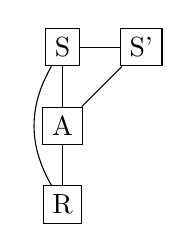
\begin{tikzpicture}[scale=.5,every node/.style={rectangle,draw}]
      \node (n6) at (1,5) {S};
      \node (n4) at (1,3) {A};
      \node (n5) at (3,5) {S'};
      \node (n1) at (1,1) {R};
      \path[every node/.style={font=\sffamily\small}]
      (n6) edge (n4)
      edge (n5)
      edge [bend right] (n1)
      (n4) edge (n1)
      edge (n5);
    \end{tikzpicture}
    \caption{MRF representation of MDP timestep}
    \label{fig:mrf}
  \end{subfigure}
  %add desired spacing between images, e. g. ~, \quad, \qquad etc. 
  %(or a blank line to force the subfigure onto a new line)
  \begin{subfigure}[b]{0.5\textwidth}
    \centering
    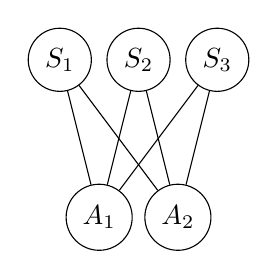
\begin{tikzpicture}[scale=.5,every node/.style={circle,draw}]
      \node (s1) at (1,5) {$S_1$};
      \node (s2) at (3,5) {$S_2$};
      \node (s3) at (5,5) {$S_3$};
      \node (a1) at (2,1) {$A_1$};
      \node (a2) at (4,1) {$A_2$};
      \path[every node/.style={font=\sffamily\small}]
      (s1) edge (a1)
      edge (a2)
      (s2) edge (a1)
      edge (a2)
      (s3) edge (a1)
      edge (a2);
    \end{tikzpicture}
    \caption{MRF sub-node decomposition}
    \label{fig:decomp}
  \end{subfigure}
  \caption{The Markov Decision Process is divided into single timestep experiences each of which can be interpreted as a Markov Random Field by discarding directionality of edges. Each cluster $S,A,R,S'$ may contain many individual nodes. Nodes are fully connected between connected clusters but disconnected within each cluster.}
  \label{fig:structure}
\end{figure}

An exponential family may be defined over the graph in Figure \ref{fig:structure} by introducing potential functions $\phi(X)$ over the nodes and edges. Equation \ref{eqn:exp-family} defines the probability of an assignment $x$ nodes the nodes in the graph given the parameters $\theta$ over nodes and edges. This is derived from the Potts model described in Wainwright and Jordan \cite{wainwright08} using the standard overcomplete representation in which the potential functions $\phi$ take the form of indicator functions over discrete values $\mathcal{X}$ (Equations \ref{eqn:node-ind}-\ref{eqn:edge-ind}).

\begin{equation}
\label{eqn:exp-family}
p(x;\theta)
=
\textrm{exp}\left\{\sum_{s \in V}\theta_{s;j}(X_s) + \sum_{(s,t) \in E} \theta_{st;jk}(X_s,X_t) - A(\theta)\right\}
\end{equation}

\begin{equation}
\label{eqn:normalization}
A(\theta)
=
\textrm{log} \sum_{X \in \mathcal{X}^m} \textrm{exp}\left\{\sum_{s \in V}\theta_{s;j}(X_s) + \sum_{(s,t) \in E} \theta_{st;jk}(X_s,X_t)\right\}
\end{equation}

\noindent\begin{minipage}{.4\linewidth}
\begin{equation}
\label{eqn:node-theta}
\theta_{s;j}(X_s) = \sum_{j \in \mathcal{X}} \theta_{s;j} \mathbb{I}_{s;j}(X_s)
\end{equation}
\end{minipage}%
\begin{minipage}{.6\linewidth}
\begin{equation}
\label{eqn:edge-theta}
\theta_{st;jk}(X_s,X_t) = \sum_{jk \in \mathcal{X} \times \mathcal{X}} \theta_{st;jk} \mathbb{I}_{st;jk}(X_s,X_t)
\end{equation}
\end{minipage}

\noindent\begin{minipage}{.4\linewidth}
\begin{equation}
\label{eqn:node-ind}
\mathbb{I}_{s;j}(X_s) = \left\{ \begin{array}{rl}
 1 &\mbox{ if $x_s = j$} \\
 0 &\mbox{ otherwise}
\end{array} \right.
\end{equation}
\end{minipage}%
\begin{minipage}{.6\linewidth}
\begin{equation}
\label{eqn:edge-ind}
\mathbb{I}_{st;jk}(X_s,X_t) = \left\{ \begin{array}{rr}
 1 &\mbox{ if $x_s = j, x_t = k$} \\
 0 &\mbox{ otherwise}
\end{array} \right.
\end{equation}
\end{minipage}

\section{Domain}
The experimental domain selected was a 9x9 gridworld pictured in Figure \ref{fig:gridworld}. The gridworld is an MDP in which the agent's state is fully described by its position $A$ in the two-dimensional world and its objective is to reach the goal state $G$. The agent takes actions corresponding to movement in any of the four cardinal directions. Each action deterministically moves the agent in the corresponding direction unless the agent has reached the edges of the grid. In this case, no further movement is possible. A reward of 1 is received when the agent reaches the goal state, 0 otherwise. More than simply specifying the dynamics of the domain, the next section describes the specific state, action, and reward representation.

\begin{figure}
\center
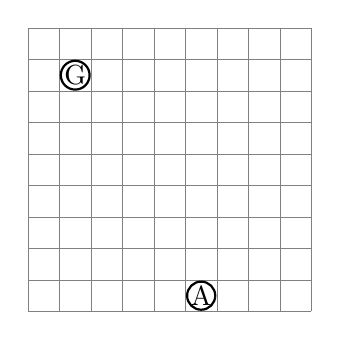
\begin{tikzpicture}[scale=.4,inner sep=0pt,thick,
    dot/.style={fill=blue,circle,minimum size=3pt}]
    \draw[help lines] (0,0) grid (9,9);
    \node[circle,draw] at (5.5,.5) {A};
    \node[circle,draw] at (1.5,7.5) {G};
\end{tikzpicture}
\caption{9x9 Gridworld. A and G respectively represent the agent and goal.}
\label{fig:gridworld}
\end{figure}

\subsection{Graph Instantiation}
The state of the system is fully described by the agents $(x,y)$ location in the world. This state is represented using 9 binary nodes to indicate which row the agent currently occupies and 9 binary nodes to represent the agent's current column. Hence, at any point in time exactly two of the state variables are active. Each of the four directional actions is encoded using using two binary nodes whose joint configuration specifies which action is to be taken (eg $0,0=\leftarrow, 0,1=\rightarrow, 1,0=\uparrow, 1,1=\downarrow$). Rewards are encoded using only a single binary node which is active when the agent reaches the goal state and inactive otherwise. When converted into the graphical representation described in Figure \ref{fig:structure}, the resulting graph contains a total of 39 vertexes (18 state nodes, 18 next state nodes, 2 action nodes, and a single reward node) and 416 edges. Parameterizing this graph over a binary $\mathcal{X}$ according to the exponential family given in Equation \ref{eqn:exp-family} yields a total of 1742 indicator function sufficient statistics and parameters. Having specified the dynamics of the MDP as well as its graphical instantiation, the next section discusses how to use this model to estimate the likelihood a given variable configuration.

\section{Likelihood Approximation}
Computing the likelihood of an assignment $X$ to the variables in the graph is a key step underlying both learning and control. The computational complexity associated with this operation stems from the normalization constant $A(\theta)$ in Equation \ref{eqn:normalization}. This constant sums over all $2^{1742}$ possible configurations of the sufficient statistics in the case of the graph representation described above. The intractability of explicitly computing $A(\theta)$ necessitates the use of approximation schemes. Pseudo-likelihood is one such approximation scheme which has the advantage of computationally tractable while still converging to the optimal $\theta$s as the number of data samples approaches infinity \cite{besag75}. Pseudo-likelihood approximates the probability of a data sample $X^t$ under the current parameters $\theta$ as the product of individual probabilities taken over the sufficient statistics of the model. Equation \ref{eqn:pseudolikelihood} expresses the pseudolikelihood; however, typically the log of this quantity is used in practice (Equation \ref{eqn:pseudologlikelihood}). Pseudolikelihood sidesteps the problem of computing the normalization constant because $A(\theta)$ occurs both in the numerator and denominator of Equation \ref{eqn:pseudologlikelihood} and thus cancels.

\begin{equation}
\tilde{p}(X^t,\theta) = \prod_{i=1}^{|\phi|} p(X_i = x_i^t | X_{V\setminus i} = X_{V\setminus i}^t) 
\label{eqn:pseudolikelihood}
\end{equation}

\begin{equation}
\textrm{log}\tilde{p}(X^t,\theta) = \sum_{i=1}^{|\phi|} \textrm{log}\frac{p(X = X^t)}{\sum_{j \in \mathcal{X}} p(x_i = j, X_{V\setminus i} = X_{V\setminus i}^t)}
\label{eqn:pseudologlikelihood}
\end{equation}

%% \begin{equation}
%% \textrm{log}\tilde{p}(X^t,\theta) = \sum_{i=1}^{|\phi|} \frac{\textrm{exp}\{\sum_{s \in V}\theta_{s;j}(X_s^t) + \sum_{(s,t) \in E} \theta_{st;jk}(X_s^t,X_t^t)\}} {\sum_{j \in \mathcal{X}}\textrm{exp}\{\sum_{s \in V}\theta_{s;j}(X_s=j) + \sum_{(s,t) \in E} \theta_{st;jk}(X_i=j,X_t^t)\}}
%% \label{eqn:fullpsuedolikelihood}
%% \end{equation}

\subsection{Optimizations to Pseudo-Likelihood}
Craig do you want to put some of your derived likelihood equations here?

Efficient likelihood approximation paves the way for tractable learning and inference, as discussed in the next section.

\section{Learning Thetas}
Learning parameters of exponential families is an area of ongoing research in the graphical model community. The formal problem definition is as follows: given a collection of fully observed data $X_1^n := {X^1...X^n}$ where each $X^i$ is a vector specifying a complete assignment of values to the sufficient statistics in the exponential family, find an assignment to the values of the unknown parameter vector $\theta$ maximizing the likelihood of the data. This is equivalent to maximizing the log of the likelihood (approximated here using the pseudolikelihood), given in Equation \ref{eqn:mle}.

\begin{equation}
\arg\max_\theta \ell(\theta,X_i^n)
=
\left\{
  \frac{1}{\textrm{n}}\sum_{i=1}^{n}\textrm{log}\tilde{p}(X^i; \theta)
\right\}
\label{eqn:mle}
\end{equation}

Wainright et al. describe a closed form solution for deriving the maximum likelihood estimate of $\theta$ \cite{wainwright08}. Unfortunately it is only applicable to triangulated graphs. While the cluster graph shown in Figure \ref{fig:mrf} is triangulated, the complete graph contains chordless cycles between adjacent layers such as Figure \ref{fig:decomp}. As a result, an iterative method must be used to learn the optimal $\theta$s. Like many optimization problems, a gradient is required for efficient maximization. The gradient of the pseudolikelihood with respect to $\theta$ is computed using automatic differentiation in Theano \cite{bergstra10} and minimized using iterative conjugate gradient \cite{hestenes52}. As these algorithms are reasonably standardized and no implementation specific alterations were made, the reader is encouraged to delve into the source code and references for further details on automatic differentiation and conjugate gradient.

\section{Results - Learning}
50 data samples were collected from an random agent (``expert'') on the 9x9 Gridworld. These data samples were divided into 2 mini-batches of size 25, with another 50 samples were set apart for evaluation. Conjugate gradient optimization took place iteratively over the samples in the two mini batches. Figure \ref{fig:learning} shows the Average un-normalized probability of data samples from the random agent compared to the probability of random initializations of the state variables. Randomly initialized states variables encode transitions and rewards which are not possible in the Gridworld MDP, such as an agent teleporting between non-adjacent grid cells or getting reward when not reaching the goal. Hence, the increased likelihood of the on-policy samples demonstrates that the learned model favors trajectories resembling the ones against which it has been trained as opposed to ``imaginary'' transitions not possible in the MDP. These results are encouraging as they indicate the presence of successful model learning. The next section addresses the challenge of making use of the learned parameters.

\begin{figure}
  \centering
  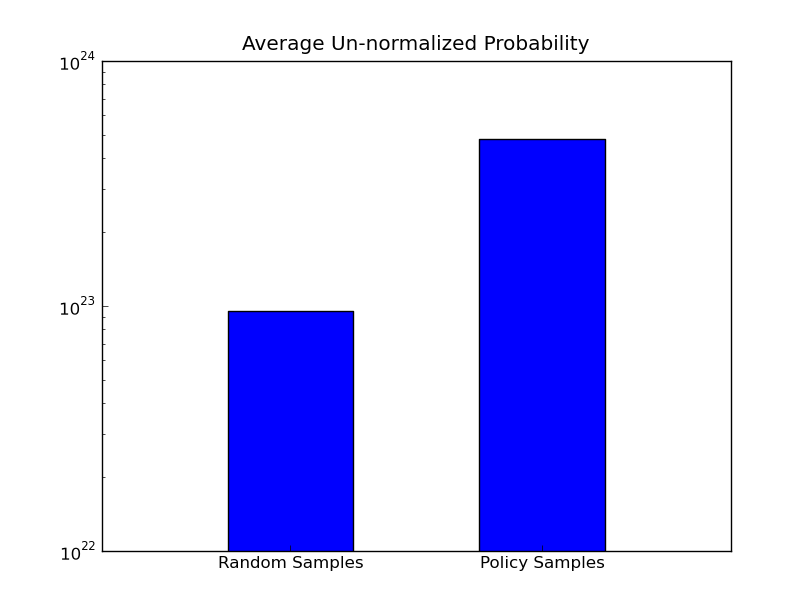
\includegraphics[width=.7\textwidth]{figures/graph.png}
  \caption{Log-scaled probability of the data sampled from a random policy (Policy Samples) and random initializations of state variables (Random Samples). This indicates that the learned model favors data generated from the policy on which it was trained to random node-wise initializations.}
  \label{fig:learning}
\end{figure}



\section{Control}

Control in reinforcement learning typically involves to finding a policy which maximizes the long term gamma discounted sum of rewards \cite{sutton98}. However, since pure imitation learning focuses instead on mimicing the expert's policy, the task becomes a supervised one where the agent is trained on $(S,R,S')$ instances whose labels are the expert's actions $A$. While training in exponential families does not involve explicitly differentiating subsets of variables as classification labels, the underlying principles are similar. During evaluation, the objective is to identify the action that the expert would most likely have taken. Fortunately, graphical models have a natural way to perform this estimation task: the Maximum a Posteriori or MAP configuration refers to the maximally likely assignment of values to the sufficient statistics in the case of exponential families or nodes in the case of graphical models. Specifically, the goal is to find the configuration $x$ maximizing $p(x,\theta)$ which is equivalent to maximizing the inner product of the parameters and the sufficient statistics (Equation \ref{eqn:map}). Note that since $A(\theta)$ does not depend on $x$ it may be ignored. Furthermore, Wainwright and Jordan \cite{wainwright08} prove that the variable configuration maximizing the inner product of parameters and sufficient statistics is equivalent to the $\mu$ maximizing the boundary set of the marginal polytope $\bar{\mathcal{M}}$ (Equation \ref{eqn:equiv}). Thus the problem becomes one of finding the $\mu$ maximizing the inner product subject to the constraints of the marginal polytope. This problem is framed as a linear program in Equation \ref{eqn:lp}. Note that there are additional constraints added beyond those of the marginal polytope: these constraints enforce that the values of the variables corresponding to the state nodes in the graph are equal to observed state in the current timestep.

\begin{equation}
\argmax_{x \in \mathcal{X}^m} p(x,\theta) = \argmax_{x \in \mathcal{X}^m} \langle \theta, \phi(x) \rangle
\label{eqn:map}
\end{equation}

\begin{equation}
\max_{x \in \mathcal{X}^m} \langle \theta,\phi(x) \rangle = \max_{\mu \in \bar{\mathcal{M}}} \langle \theta, \mu \rangle
\label{eqn:equiv}
\end{equation}

\begin{equation}
\begin{array}{llr}
\textrm{Maximize: } & \langle \theta, \mu \rangle & \textrm{(objective)}\\
\textrm{Subject to: } & \sum_{x_i \in \mathcal{X}} \mu_i(x_i) = 1 & \textrm{(node-wise constraints)}\\
& \sum_{x_j \in \mathcal{X}} \mu_{ij}(x_i,x_j) = \mu_i(x_i) & \textrm{(edge-wise constraints)}\\
& x_s = X_s^t \textrm{ } \forall s \in \textrm{state nodes} & \textrm{(observed state constraints)}
\end{array}
\label{eqn:lp}
\end{equation}

Unfortunately, the linear program expressed in Equation \ref{eqn:lp} is only guaranteed to be integral in the case tree structured Markov Random Fields over discrete random variables. It is possible to enforce integral solutions by solving the corresponding integer program (IP), however integer programs are NP-hard in general. One solution to this problem is to round the real-valued $\mu$ returned by the linear program. Curiously, in the case of this work it was found that the $\mu$ returned by the lp was indeed integral, so no rounding was necessary.

%This work utilizes a na\"{\i}ve rounding scheme in which real-values are rounded to the nearest discrete value in $\mathcal{X}$. Because the action nodes are the nodes of greatest interest and each possible configuration of action nodes corresponds to a legitimate action in the MDP, this na\"{\i}ve rounding scheme is guaranteed to return interpretable results. The next section delves into results obtained on the Gridworld domain using this control mechanism.

\section{Results - Control}
Control experiments were carried out on the 9x9 Gridworld. The first experiment  learning from data produced by an optimal agent and quantifying how much reward was received compared to the optimal agent. Figure \ref{fig:reward} shows the cumulative reward of the agent compared with that of the optimal agent.

\begin{figure}
  \centering
  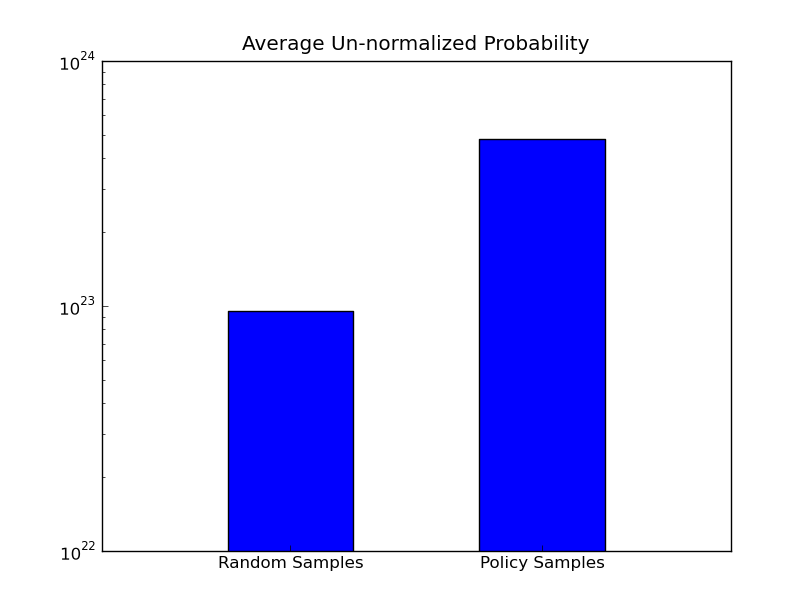
\includegraphics[width=.7\textwidth]{figures/graph.png}
  \caption{This graph should show how much reward the agent collects compared to the optimal agent}
  \label{fig:reward}
\end{figure}


Next the similarity between the learned policy $\pi$ and the experts policy $\bar{\pi}$ is examined as a function of the number of training data samples which were provided. Let us define the Policy Similarity of two policies in an MDP with a finite number of states and discrete actions as the percentage of states in which the policies choose the same action to execute. This quantity is defined formally in Equation \ref{eqn:policysim}. Figure \ref{fig:policysim} depicts the rate a which the similarity between the learned policy and the expert's policy grows.

\begin{equation}
\begin{array}{l}
\textrm{Policy Similarity}(\pi,\pi') = \frac{1}{|S|}\sum_{s \in S} \mathbb{I}(\pi(s),\pi'(s)) \\
\\
\mathbb{I}(\pi(s),\pi'(s)) = \left\{ \begin{array}{rl}
 1 &\mbox{ if $\pi(s) = \pi'(s)$} \\
 0 &\mbox{ otherwise}
\end{array} \right. \\
\end{array}
\label{eqn:policysim}
\end{equation}

\begin{figure}
  \centering
  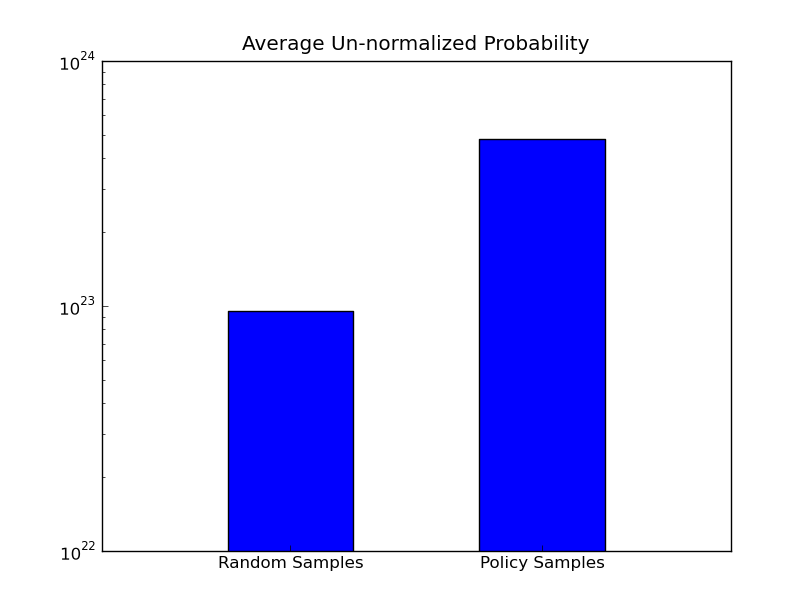
\includegraphics[width=.7\textwidth]{figures/graph.png}
  \caption{This graph should show how the policy gets more similar as the size of the training data samples increases.}
  \label{fig:policysim}
\end{figure}


\section{Future Work}
There are many avenues of future work. One of the first possibilities would involve extending the graphical model to include more than a single time step in the MDP. Full trajectories could encompass arbitrarily many timesteps so graph size is theoretically unbounded. However, the discount factor $\gamma$ specifies a horizon beyond which rewards matter little. Therefore it would likely be possible to compute, given a setting for $\gamma$, the minimum size of the graph necessary to ensure learning converges within some constant factor of optimality. 

Another promising avenue of future work is to introduce a hidden component to the graph:

\makebox[\textwidth][c]{
  \centering
  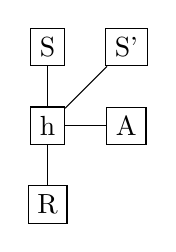
\begin{tikzpicture}[scale=.5,every node/.style={rectangle,draw}]
    \node (n6) at (1,5) {S};
    \node (n4) at (3,3) {A};
    \node (n0) at (1,3) {h};
    \node (n5) at (3,5) {S'};
    \node (n1) at (1,1) {R};
    \path[every node/.style={font=\sffamily\small}]
    (n0) edge (n1)
    edge (n1)
    edge (n5)
    edge (n4)
    edge (n6);
  \end{tikzpicture}
}

This hidden component could include various amounts of representational power by varying the number and topology the nodes contained within. 

Another interesting vein of future work is to apply algorithms developed in the deep learning community to the graphical structure described in Figure \ref{fig:structure}. Because of the connectivity each cluster of nodes forms a fully connected bipartite graph with every other cluster. This structure is identical to that found in Restricted Boltzmann Machines, the building blocks of deep nets \cite{ackley85}. Extensive work has been already done in the deep learning community to develop efficient algorithms for learning and inference in the deep nets. Algorithms such as Contrastive Divergence \cite{hinton02} apply directly to the topology of this problem. 

\section{Discussion and Conclusion}
This work applied graphical model and exponential family algorithms to the problem of pure imitation learning in Markov Decision Processes. It was demonstrated that the graph structure of a single MDP timestep could be decomposed into a Markov Random Field. Given a collection of data from an expert, this paper described the application of the psuedolikelihood approximation for estimating the likelihood of arbitrary graph configurations. Combining this likelihood estimation procedure with an automatically derived gradient, allowed the efficient use of conjugate descent to learn parameters to maximize the likelihood of the training data. Learned parameters were empirically shown to successfully increase the likelihood of on-policy samples when compared to to random samples. Subsequently, control could be performed through inferring the Maximum a Posteriori (MAP) configuration of variables in the graph for the current timestep. The resulting policy was shown to excel at recreating the expert's policy even when provided with samples far fewer than the number of possible states in the system. 

\bibliography{gm-control}
\bibliographystyle{plain}
\end{document}
